
\documentclass[tikz]{standalone}
\usepackage{graphicx}
\usepackage{lmodern}
\usepackage{amsmath, amssymb, amsfonts}
\usetikzlibrary{calc}
\newcommand{\R}{\mathcal{R}}

\definecolor{blue1}{rgb}{0.6,0.8.,1.}
\definecolor{blue2}{rgb}{0.4,0.6,1.}
\definecolor{blue3}{rgb}{0.2,0.4,1.}
\definecolor{blue4}{rgb}{0,0,1}

\begin{document}

%n = 5, d = 2 construction proof intuition for abstain
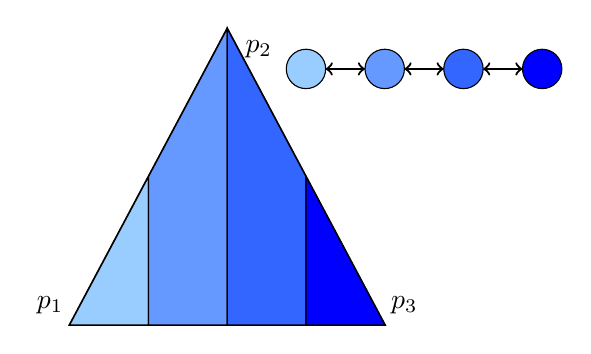
\begin{tikzpicture}
\coordinate (p1) at (-2,0);
\coordinate (p2) at (0,3.76);
\coordinate (p3) at (2,0);

\coordinate (p1p2) at (-1, 3.76/2);
\coordinate (p2p3) at (1, 3.76/2);

\draw[thick] (p1) -- (p2) -- (p3) -- cycle;
\draw[fill = blue1] (p1) -- (p1p2) -- (-1,0) -- cycle;
\draw[fill = blue2] (p1p2)-- (p2) -- (0,0) -- (-1,0) -- cycle;
\draw[fill = blue3] (p2p3)-- (p2) -- (0,0) -- (1,0) -- cycle;
\draw[fill = blue4] (p2p3)-- (p3) -- (1,0) -- cycle;


%label point distributions
%label outcomes
\node at (-9/4, 1/4) {$p_1$};
\node at (2/5, 3.5) {$p_2$};
\node at (9/4, 1/4) {$p_3$};

%graph underneath simplex
\draw [fill = blue1] (1., 3.25) circle (0.25);
\draw [fill = blue2] (2., 3.25) circle (0.25);
\draw [fill = blue3] (3., 3.25) circle (0.25);
\draw [fill = blue4] (4., 3.25) circle (0.25);
\draw[<->, thick] (1.25, 3.25) -- (1.75, 3.25);
\draw[<->, thick] (2.25, 3.25) -- (2.75, 3.25);
\draw[<->, thick] (3.25, 3.25) -- (3.75, 3.25);

\end{tikzpicture}


\end{document}
%%% Local Variables:
%%% mode: latex
%%% TeX-master: t
%%% End:
